\chapter{Aufgaben im Labor}
\thispagestyle{fancy}

\section{Theoretische Lösung aus V1}

Die theoretische Ausgangsfunktion $u_y(t)$ soll mit Matlab programmiert und in einem Grafen dargestellt werden. 

\vspace{0.5cm}

\begin{lstlisting}
%% Aufgabe 1

% Berechnung der Lade- und Entladekurve

t1 = 0:dt:tau;              % Ladezeit
uy1 = U * (1-exp(-t1/tau)); % Ladefunktion

t2 = tau:dt:(tau+5*tau);    % Entladezeit
uy2 = U * (1-exp(-tau/tau)) * exp(-(t2-tau)/tau); % Entladefkt

uy = [uy1, uy2];    % Zusammensetzen der Lade- und Entladewerte
t = [t1, t2];

plot(t, uy); grid on; grid minor; %axis tight; 

% Beschriftung des Graphen:

title('Ausgangsspannung u_y(t)');
xlabel('t');
ylabel('u_y(t)');

\end{lstlisting}

\vspace{0.5cm}
    
Ausgegeben wird folgende Grafik:
\begin{center}
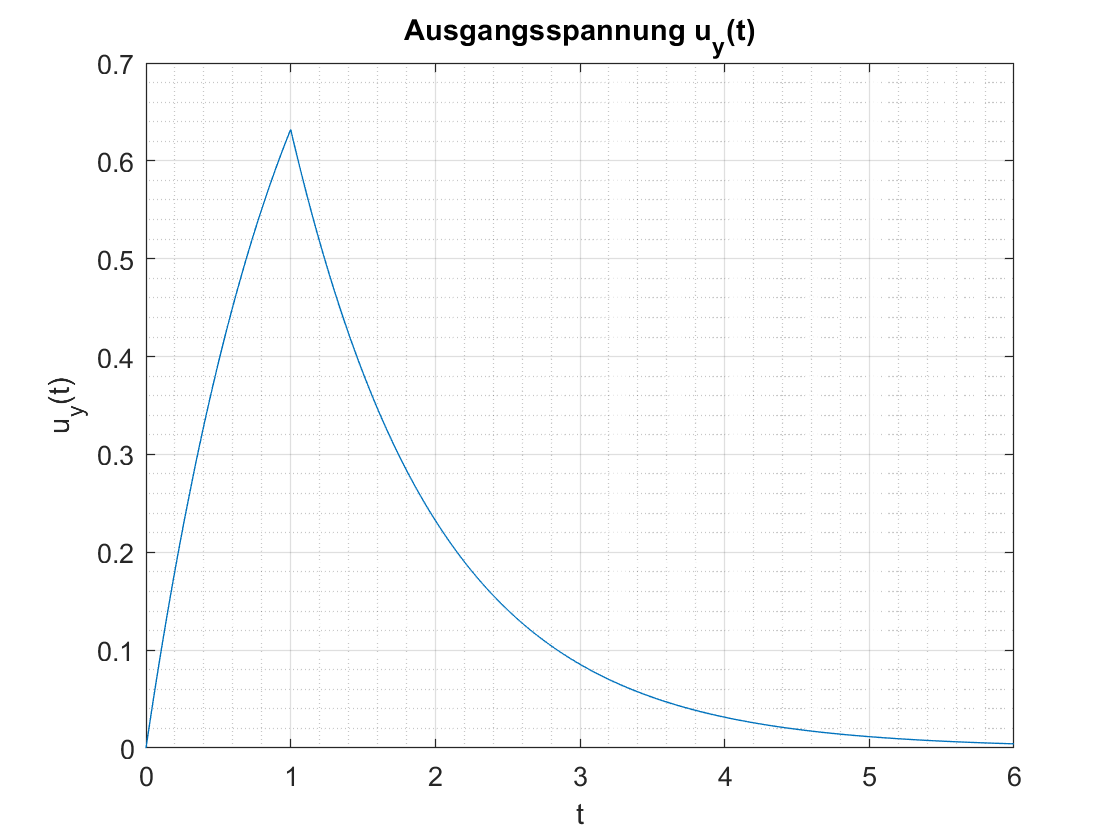
\includegraphics[width=200pt]{img/aufgabe1.png}
\end{center}

